% tetrahedron.tex

%%%%%%%%%%%%%%%%%%%%
\begin{frame}
  \fig{width = 0.30\textwidth}{figs/tetrahedron}

  \[
	\sym(T) \cong \pause \red{A_4}
  \]

  \pause
  \vspace{-0.30cm}
  \[
	\Big\lvert \big\{H: H \le \sym(T)\big\} \Big\rvert = \pause \red{10}
  \]
\end{frame}
%%%%%%%%%%%%%%%%%%%%

%%%%%%%%%%%%%%%%%%%%
\begin{frame}
  \fig{width = 0.25\textwidth}{figs/tetrahedron}

  \[
	\red{\sym(T) \cong A_4}
  \]

  \pause
  \begin{proof}
	\begin{enumerate}[(1)]
		\centering
	  \item To find all \purple{even} perms. in $S_4$ 
		\pause
	  \item To show that $\Big\lvert \sym(T) \Big\rvert < \Big\lvert S_4 \Big\rvert$
	\end{enumerate}
  \end{proof}
\end{frame}
%%%%%%%%%%%%%%%%%%%%

%%%%%%%%%%%%%%%%%%%%
\begin{frame}
  \fig{width = 0.25\textwidth}{figs/tetrahedron}

  \[
	\Big\lvert \sym(T) \Big\rvert < \Big\lvert S_4 \Big\rvert
  \]

  \pause
  \[
	\because (1\; 2) \notin \sym(T)
  \]
\end{frame}
%%%%%%%%%%%%%%%%%%%%

%%%%%%%%%%%%%%%%%%%%
\begin{frame}
  \fig{width = 0.50\textwidth}{figs/tetrahedron}
  \vspace{-1.00cm}
  \begin{center}
	{\it Clockwise}
  \end{center}
\end{frame}
%%%%%%%%%%%%%%%%%%%%

%%%%%%%%%%%%%%%%%%%%
\begin{frame}
  \begin{center}
	Rotate through vertices:
  \end{center}

  \begin{align*}
	\text{Fixing } 1: \rho_{1} = (2\; 3\; 4)\quad \rho_{1}^{2} = (2\; 4\; 3)\quad \rho_{1}^{3} = 1 \\[6pt]
	\text{Fixing } 2: \rho_{2} = (1\; 3\; 4)\quad \rho_{2}^{2} = (1\; 4\; 3)\quad \rho_{2}^{3} = 1 \\[6pt]
	\text{Fixing } 3: \rho_{3} = (1\; 2\; 4)\quad \rho_{3}^{2} = (1\; 4\; 2)\quad \rho_{3}^{3} = 1 \\[6pt]
	\text{Fixing } 4: \rho_{4} = (1\; 2\; 3)\quad \rho_{4}^{2} = (1\; 3\; 2)\quad \rho_{4}^{3} = 1
  \end{align*}

  \pause
  \[
	\blue{\# = 8 + 1 = 9}
  \]
\end{frame}
%%%%%%%%%%%%%%%%%%%%

%%%%%%%%%%%%%%%%%%%%
\begin{frame}
  \begin{center}
	Rotate through edge-edge:
  \end{center}

  \begin{align*}
	r_1 = (1\; 4) (2\; 3) \\[6pt]
	r_2 = (1\; 2) (3\; 4) \\[6pt]
	r_3 = (1\; 3) (2\; 4)
  \end{align*}

  \pause
  \[
	\blue{\# = 3}
  \]
\end{frame}
%%%%%%%%%%%%%%%%%%%%

%%%%%%%%%%%%%%%%%%%%
\begin{frame}
  \begin{columns}
	\column{0.60\textwidth}
	  \begin{align*}
		\rho_{1} = (2\; 3\; 4)\quad \rho_{1}^{2} = (2\; 4\; 3) \\[3pt]
		\rho_{2} = (1\; 3\; 4)\quad \rho_{2}^{2} = (1\; 4\; 3) \\[3pt]
		\rho_{3} = (1\; 2\; 4)\quad \rho_{3}^{2} = (1\; 4\; 2) \\[3pt]
		\rho_{4} = (1\; 2\; 3)\quad \rho_{4}^{2} = (1\; 3\; 2)
	  \end{align*}
	\column{0.40\textwidth}
	  \begin{align*}
		r_1 = (1\; 4) (2\; 3) \\[6pt]
		r_2 = (1\; 2) (3\; 4) \\[6pt]
		r_3 = (1\; 3) (2\; 4)
	  \end{align*}
  \end{columns}

  \vspace{0.60cm}
  \[
	\red{\boxed{\sym(T) \cong A_4 = \set{\text{id},\quad \underbrace{\text{3-cycle}}_{\# = 8},\quad \underbrace{\text{2-2-cycle}}_{\# = 3}}}}
  \]
\end{frame}
%%%%%%%%%%%%%%%%%%%%

%%%%%%%%%%%%%%%%%%%%
\begin{frame}
  \[
	\red{\boxed{\Big\lvert \big\{H: H \le \sym(T)\big\} \Big\rvert = 10}}
  \]

  \pause
  \[
	H \le A_4 \red{\implies} \bcard{H} = 1, 2, 3, 4, 6, 12
  \]

  \pause
  \[
	\bcard{H} = \begin{cases}
	  1: & \text{id} \quad \blue{(\# = 1)} \\[3pt]
	  2: & \gen{r_1}, \gen{r_2}, \gen{r_3} \quad \blue{(\# = 3)} \\[3pt]
	  3: & \gen{\rho_1}, \gen{\rho_2}, \gen{\rho_3}, \gen{\rho_4} \quad \blue{(\# = 4)} \\[3pt]
	  4: & \violet{\set{1, r_1, r_2, r_3} \cong K_4} \quad \red{(\# = 1)} \\[3pt]
	  6: & \red{(\# = 0)} \\[3pt]
	  12: & A_4 \quad \blue{(\# = 1)}
	\end{cases}
  \]

  % \[
  %   \bcard{H} = \begin{cases}
  %     1: & \pause \text{id} \quad \blue{(\# = 1)} \\[3pt] \pause
  %     2: & \pause \gen{r_1}, \gen{r_2}, \gen{r_3} \quad \blue{(\# = 3)} \\[3pt] \pause
  %     3: & \pause \gen{\rho_1}, \gen{\rho_2}, \gen{\rho_3}, \gen{\rho_4} \quad \blue{(\# = 4)} \\[3pt]
  %     4: & \pause \violet{\set{1, r_1, r_2, r_3} \cong K_4} \quad \red{(\# = 1)} \\[3pt] \pause
  %     6: & \pause \red{(\# = 0)} \\[3pt] \pause
  %     12: & \pause A_4 \quad \blue{(\# = 1)}
  %   \end{cases}
  % \]
\end{frame}
%%%%%%%%%%%%%%%%%%%%

%%%%%%%%%%%%%%%%%%%%
\begin{frame}
  \begin{theorem}[Groups of Order $4$]
	\[
	  \bcard{G} = 4 \red{\implies} G \cong \z_{4} \lor G \cong K_4 \cong \z_{2} \times \z_{2}
	\]
  \end{theorem}

  \pause
  \begin{columns}
	\column{0.50\textwidth}
	  \fig{width = 0.60\textwidth}{figs/z4}
	  \[
		\z_{4}
	  \]
	\column{0.50\textwidth}
	  \fig{width = 0.50\textwidth}{figs/z2xz2}
	  \[
		K_4 \cong \z_{2} \times \z_{2}
	  \]
  \end{columns}
\end{frame}
%%%%%%%%%%%%%%%%%%%%

%%%%%%%%%%%%%%%%%%%%
\begin{frame}
  \begin{theorem}[Groups of Order $4$]
	\[
	  \bcard{G} = 4 \red{\implies} G \cong \z_{4} \lor G \cong K_4 \cong \z_{2} \times \z_{2}
	\]
  \end{theorem}

  \begin{proof}
	\pause
	\[
	  \blue{\bcard{G} = 4, H \le G \implies \bcard{H} = 1, 2, 4}
	\]

	\pause
	\begin{columns}
	  \column{0.50\textwidth}
		\uncover<3->{
		  \[
			\purple{\exists a \in G: \card{a} = 4}
		  \]
		}

		\vspace{-0.50cm}
		\uncover<5->{
		  \[
			G = \gen{a} \cong \z_{4}
		  \]
		}
	  \column{0.50\textwidth}
		\uncover<4->{
		  \[
			\purple{\forall a \in G: a \neq e \implies \card{a} = 2}
		  \]
		}

		\vspace{-0.50cm}
		\uncover<6>{
		  \[
			H = \set{e, a, b, ab}
		  \]

		  \[
			a^2 = b^2 = e, ab = ba
		  \]
		}
	\end{columns}
  \end{proof}
\end{frame}
%%%%%%%%%%%%%%%%%%%%

%%%%%%%%%%%%%%%%%%%%
\begin{frame}
  \begin{theorem}[Groups of Order $6$]
	\[
	  {\bcard{G} = 6 \red{\implies} \pause G \cong \z_{6} \lor G \cong D_3}
	\]
  \end{theorem}

  \pause
  \begin{columns}
	\column{0.50\textwidth}
	  \fig{width = 0.60\textwidth}{figs/z6}
	  \[
		\z_{6}
	  \]
	\column{0.50\textwidth}
	  \fig{width = 0.65\textwidth}{figs/d3}
	  \[
		D_3
	  \]
  \end{columns}
\end{frame}
%%%%%%%%%%%%%%%%%%%%

%%%%%%%%%%%%%%%%%%%%
\begin{frame}
  \begin{theorem}[Groups of Order $6$]
	\[
	  \bcard{G} = 6 \red{\implies} G \cong \z_{6} \lor G \cong D_3
	\]
  \end{theorem}

  \pause
  \[
	\blue{\bcard{G} = 6, H \le G \implies \bcard{H} = 1, 2, 3, 6}
  \]

  \pause
  \[
	(1)\; \exists a \in G, \card{a} = 6 \implies G = \gen{a} \cong \z_{6}
  \]

  \pause
  \vspace{-0.50cm}
  \[
	(2)\; \forall a \in G, a \neq e \implies \card{a} = 2 \lor \card{a} = 3
  \]
  
  \pause
  \begin{columns}
	\column{0.40\textwidth}
	  \[
		\red{\exists a \in G: \card{a} = 2}
	  \]
	\column{0.40\textwidth}
	  \[
		\red{\exists a \in G: \card{a} = 3}
	  \]
  \end{columns}

  \pause
  \vspace{0.60cm}
  \[
	\boxed{G = \set{e, a, a^2, b, ba, ba^2} \quad \red{(a^3 = b^2 = e)}}
  \]
\end{frame}
%%%%%%%%%%%%%%%%%%%%

%%%%%%%%%%%%%%%%%%%%
\begin{frame}
  \[
	\boxed{G = \set{e, a, a^2, b, ba, ba^2} \quad \red{(a^3 = b^2 = e)}}
  \]

  \pause
  \[
	\teal{(2.1)\; ab = ba}
  \]
  \pause
  \[
	G = \gen{a, b \mid a^3 = b^2 = e, ab = ba} \cong \z_6
  \]

  \pause
  \[
	\teal{(2.2)\; ab = ba^2}
  \]
  \pause
  \[
	G = \gen{a, b \mid a^3 = b^2 = e, bab^{-1} = a^{-1}} \cong D_3
  \]
\end{frame}
%%%%%%%%%%%%%%%%%%%%

%%%%%%%%%%%%%%%%%%%%
\begin{frame}
  \begin{theorem}[Theorem $6.15$]
	$A_4$ has no subgroup of order $6$.
  \end{theorem}

  \pause
  \begin{center}
	\red{By contradiction.} \\[5pt] \pause
	\blue{Suppose that $A_4$ has a subgroup $H$ of order $6$.} \\[5pt] \pause

	\[
	  H \ncong \z_{6} \implies H \cong D_3
	\]

	\pause
	\[
	  D_3 = \set{e, a, a^2, b, ba, ba^2} \quad (a^3 = b^2 = e, bab^{-1} = a^{-1})
	\]

	\pause
	$D_3$ contains $3$ elements of order $2$.

	\pause
	$H$ contains $3$ elements of order $2$.

	\pause
	\[
	  \set{1, r_1, r_2, r_3} \subseteq H
	\]

	\pause
	\vspace{-0.60cm}
	\[
	  K_4 \cong \set{1, r_1, r_2, r_3} \le H \red{\implies 4 \mid 6}
	\]
  \end{center}
\end{frame}
%%%%%%%%%%%%%%%%%%%%

%%%%%%%%%%%%%%%%%%%%
\begin{frame}
  \fig{width = 0.30\textwidth}{figs/arthur-cayley}
  \begin{center}
	\teal{Arthur Cayley ($1821$ -- $1895$)}
  \end{center}
\end{frame}
%%%%%%%%%%%%%%%%%%%%

%%%%%%%%%%%%%%%%%%%%
\begin{frame}
  \begin{columns}
	\column{0.50\textwidth}
	  \fig{width = 0.60\textwidth}{figs/z6}
	  \[
		\z_{6}
	  \]
	\column{0.50\textwidth}
	  \fig{width = 0.70\textwidth}{figs/d3}
	  \[
		D_3
	  \]
  \end{columns}

  \pause
  \vspace{0.50cm}
  \[
	\Gamma(G, S),\quad S \text{ is a \red{generating set}}
  \]
\end{frame}
%%%%%%%%%%%%%%%%%%%%

%%%%%%%%%%%%%%%%%%%%
\begin{frame}
  \begin{columns}
	\column{0.60\textwidth}
	  \begin{align*}
		\rho_{1} = (2\; 3\; 4)\quad \rho_{1}^{2} = (2\; 4\; 3) \\[3pt]
		\rho_{2} = (1\; 3\; 4)\quad \rho_{2}^{2} = (1\; 4\; 3) \\[3pt]
		\rho_{3} = (1\; 2\; 4)\quad \rho_{3}^{2} = (1\; 4\; 2) \\[3pt]
		\rho_{4} = (1\; 2\; 3)\quad \rho_{4}^{2} = (1\; 3\; 2)
	  \end{align*}
	\column{0.40\textwidth}
	  \begin{align*}
		r_1 = (1\; 4) (2\; 3) \\[6pt]
		r_2 = (1\; 2) (3\; 4) \\[6pt]
		r_3 = (1\; 3) (2\; 4)
	  \end{align*}
  \end{columns}

  \pause
  \vspace{0.60cm}
  \[
	\blue{a = (1\; 2\; 3)} \qquad \red{b = (1\; 2) (3\; 4)}
  \]
\end{frame}
%%%%%%%%%%%%%%%%%%%%

%%%%%%%%%%%%%%%%%%%%
\begin{frame}
  \begin{center}
	\resizebox{0.70\textwidth}{!}{% a4-cayley.tex

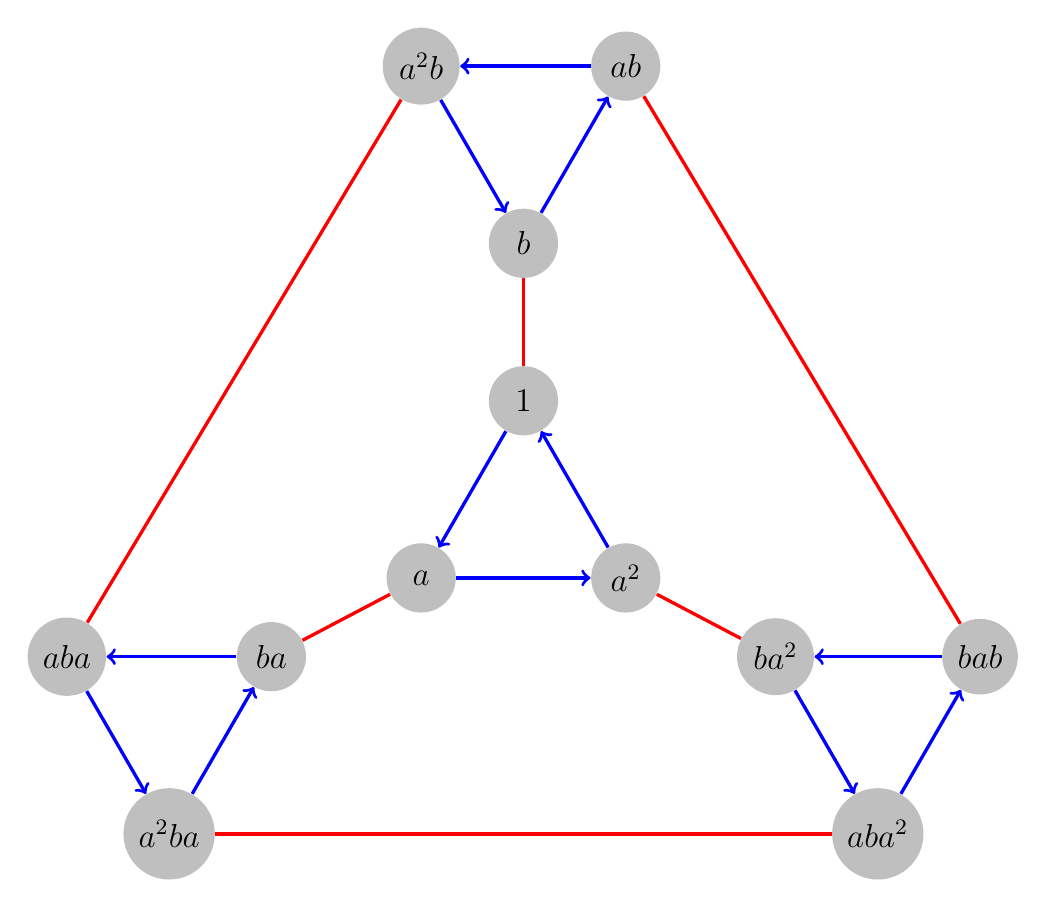
\begin{tikzpicture}[ele/.style = {circle, minimum size = 25pt, fill = lightgray, font = \large},
  a/.style = {->, blue, very thick},
  b/.style = {-, red, very thick}]
  % center 
  \foreach \angle/\label in {90/1, -30/a^2, -150/a} {
	\node (\label) [ele] at (\angle:1.5) {$\label$};
  }

  % below left
  \begin{scope}[xshift = -4.5cm, yshift = -2.5cm]
	\foreach \angle/\label in {30/ba, -90/a^2ba, -210/aba} {
	  \node (\label) [ele] at (\angle:1.5) {$\label$};
	}
  \end{scope}

  % below right
  \begin{scope}[xshift = 4.5cm, yshift = -2.5cm]
	\foreach \angle/\label in {30/bab, -90/aba^2, -210/ba^2} {
	  \node (\label) [ele] at (\angle:1.5) {$\label$};
	}
  \end{scope}

  % above
  \begin{scope}[yshift = 5.0cm]
	\foreach \angle/\label in {30/ab, -90/b, -210/a^2b} {
	  \node (\label) [ele] at (\angle:1.5) {$\label$};
	}
  \end{scope}

  \path (1) edge[a] (a)
		(a) edge[a] (a^2)
		(a^2) edge[a] (1)

		% below left
		(ba) edge[a] (aba)
		(aba) edge[a] (a^2ba)
		(a^2ba) edge[a] (ba)

		% below right
		(aba^2) edge[a] (bab)
		(bab) edge[a] (ba^2)
		(ba^2) edge[a] (aba^2)

		% above 
		(b) edge[a] (ab)
		(ab) edge[a] (a^2b)
		(a^2b) edge[a] (b)

		% b
		(1) edge[b] (b)
		(a) edge[b] (ba)
		(a^2) edge[b] (ba^2);

  \pause
  \path (a^2b) edge[b] (aba)
		(a^2ba) edge[b] (aba^2)
		(bab) edge[b] (ab);
\end{tikzpicture}
}
  \end{center}

  \vspace{-0.80cm}
  \[
	\blue{a}^3 = \red{b}^2 = 1 \only<3->{\quad (\red{b}\blue{a})^3 = 1}
  \]
\end{frame}
%%%%%%%%%%%%%%%%%%%%

%%%%%%%%%%%%%%%%%%%%
\begin{frame}
  \fig{width = 0.50\textwidth}{figs/a4-cayley-in-tetrahedron}

  \begin{center}
	$\sym(T) \cong A_4$ arranged on a \red{\it truncated} tetrahedron
  \end{center}
\end{frame}
%%%%%%%%%%%%%%%%%%%%
